%To be able to convey semantically meaningful commands through the use of gestures one relies on gesture recognition systems, 
%which is responsible for capturing and interpreting gestures from the user and carry out the desired action. 
To be able to apply the various hand gesture recognition algorithms one must first be able to monitor the user hands through some sort of hardware. 
There are several categories of these recognition systems, which usually have roots in sensor technology, 
image processing and computer vision~\citep{Vafadar2014}.

The first attempts at a commercial hand gesture recognition system were typically glove-based control interfaces, often called \textit{data gloves},
and were gloves with sensors attached to it. As the image processing and computer vision technology wasn't mature yet, these \textit{contact-based devices} remained 
the primary gesture recognition technology until the image processing-reliant \textit{vision-based devices} began to see some success in the 2000s~\citep{Premaratne2014}.
Another factor that made data gloves ideal was a very limited requirement for processing power, as any pre-processing were rarely done, 
and thus the systems could run optimally on the commodity 1980s and 1990s computers~\citep{Premaratne2014}.  

% Gesture recognition technology is a field that has gained much attention with the growth of the virtual reality field, 
% and it's a very diverse one with roots in sensor technology, image processing and computer vision~\citep{Vafadar2014}.

\begin{figure}%[h!] %[H]
	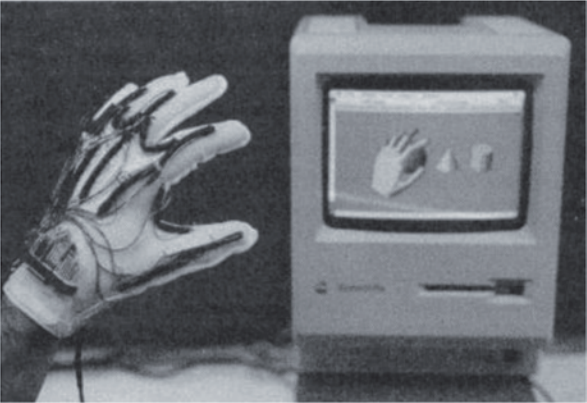
\includegraphics[width=\linewidth]{pictures/old_dataglove.png}
	\caption[The Z Glove]{The Z Glove, developed by Zimmerman in 1982. Picture from \citet{Premaratne2014}}
	\label{fig:old_dataglove}
\end{figure} 

Today, both contact-based and vision-based devices are utilized for gesture recognition purposes. 
The following subsections will the discuss the main properties of the two and review their differences.

\subsection{Contact-based Devices} 
Contact-based devices are usually wearable objects, such as gloves or armbands, 
which register the user's kinetic movement through sensors. %and attempt to mirror it in the virtual world. 
A variety of sensor technologies have been applied to capture the physical data of a users hand (such as finger bending and hand orientation and position).
Traditionally a combination of \textit{inertial navigation systems}\footnote{A navigation tool, often used on ships and aircrafts, that calculates position, orientation and velocity.} 
and \textit{flex sensors}\footnote{A "bend sensor" that measure the amount of deflection.} have been utilized in contact-based gesture recognition devices~\citep{Sturman1994}. 
Inertial navigation systems contain motion and rotation sensors, such as accelerometers and gyroscopes, and is used to monitor the hand position and orientation by
calculating the position, orientation and velocity (in terms of direction and speed) via \textit{dead reckoning}, and thus without the need for external references~\citep{Berg1970}.
Flex sensors are often positioned at important finger joint to determine the amount the finger is bent by. 

There are also other types of sensors being used in various contact-based products. 
One example of this is the Myo armband by Thalmic Labs (see figure~\vref{fig:myo}), which - in addition to containing gyroscopes, accelerometers and magnetometers - also utilizes 
a set of electromyographic (EMG)
\footnote{Electromyography (EMG) is an electrodiagnostic medicine technique for evaluating and recording the electrical activity produced by skeletal muscles~\citep{Kamen2004}}
sensors that sense electrical activity in the forearm muscles~\citep{Myo2015} 
By monitoring this electrical activity, i.e the electric potential of the muscles, the Myo armband can thus determine the state of each muscle (e.g~whether it is contracted or not).


\begin{figure}%[h!] %[H]
	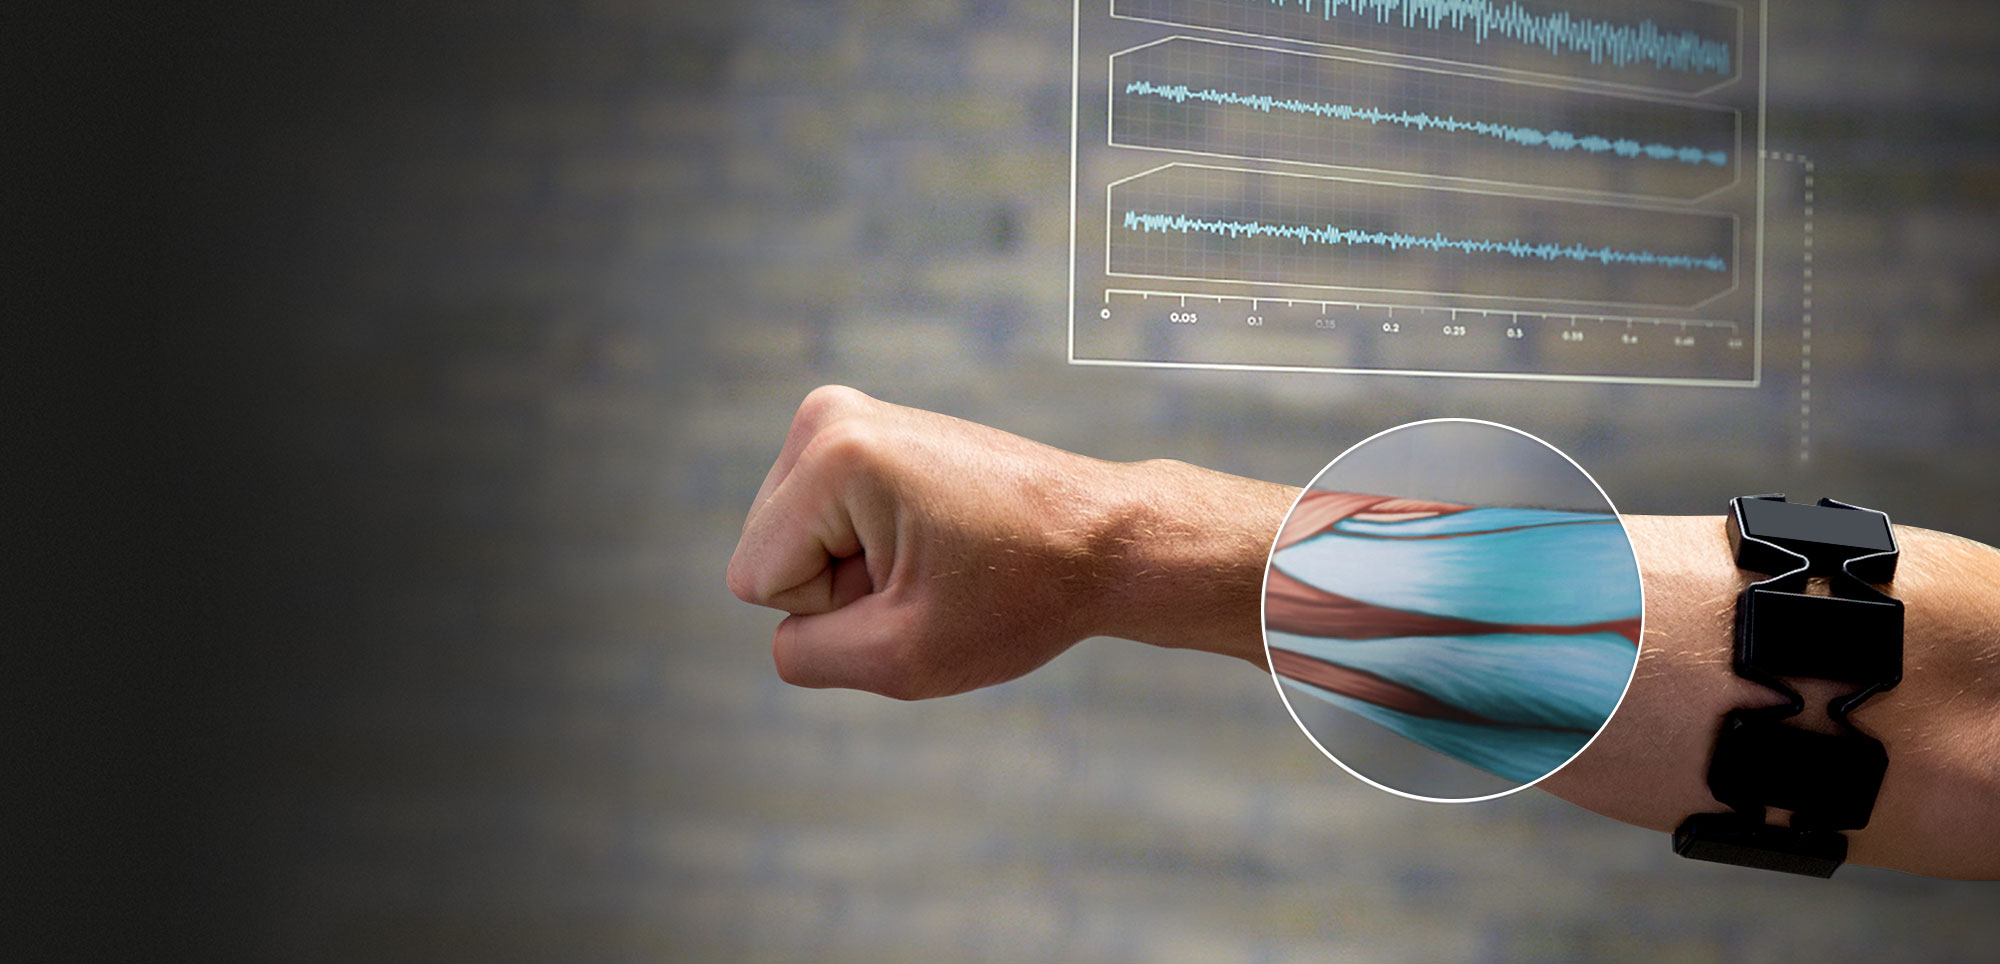
\includegraphics[width=\linewidth]{pictures/myo_armband.jpg}
	\caption[The Myo armband]{The Myo armband is a contact-based gesture recognition device worn on the forearm. Picture from~\citet{Myo2015}.}
	\label{fig:myo}
\end{figure}

\subsection{Vision-based Devices} 
Vision-based devices usually make use of either depth-aware cameras or stereo cameras to approximate a contour/silhouette or 
3D representation of what's output by the cameras. A vision-based hand gesture recognition system thus takes "pictures"\footnote{Usually about 60 images/frames per second} of the 
user's hands, and often applies various image processing techniques (e.g image normalization) before using a computer vision algorithm to detect if any known gesture is 
being performed. Today, there are three primary vision-based technologies: \textit{Stereoscopic vision}, \textit{structured light} and 
\textit{time of flight}~\citep{Ko2012} (see figure~\vref{fig:VBComparisions} for a comparison). 
These technologies all use different techniques to construct 3D representations of the captured 2D images, as the 
depth information is crucial in a vision-based gesture recognition system~\citep{Ko2012}.

\begin{figure}%[h!] %[H]
	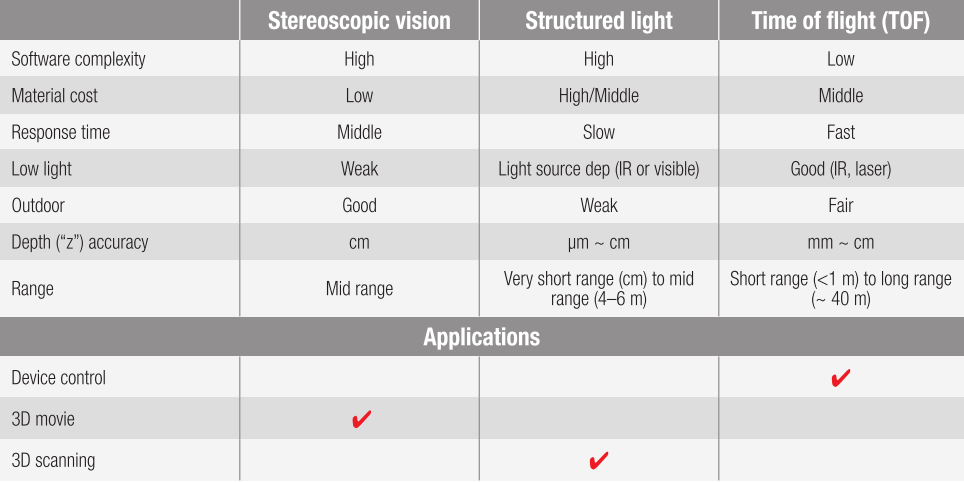
\includegraphics[width=\linewidth]{pictures/Vision-based_comparisons.png}
	\caption{Comparison of Vision-based sensor technologies~\citep{Ko2012}.}
	\label{fig:VBComparisions}
\end{figure} 

Stereoscopic vision is arguably the most common of these vision-based methods and is a method that in many ways seem inspired by how the human body processes depth information.
This technique uses two cameras - often referred to as a stereo camera - to obtain a left and right image (just as human eyes), which are sent to
the tracking software. After such a stereo image (see figure~\vref{fig:stereo_image}) is captured the left- and right part are compared in software and a disparity image that relates the 
displacement of objects in the images is created. This disparity image can in many ways be regarded as a sum of the offsets between the left and right images,
due to their cameras' different point of views of the tracked object. 

\begin{figure}%[h!] %[H]
	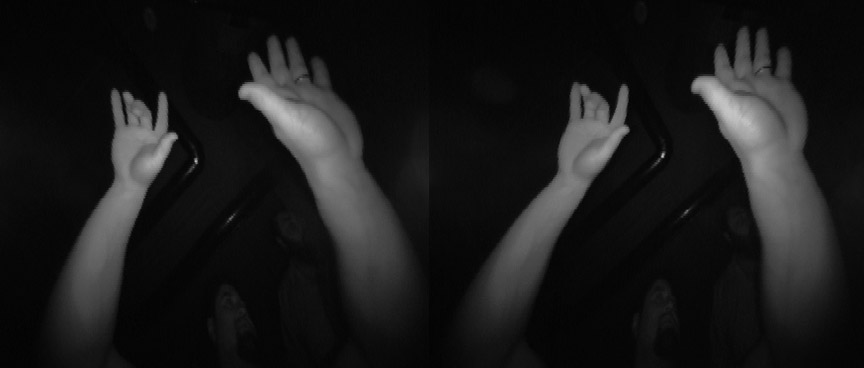
\includegraphics[width=\linewidth]{pictures/stereo_image.jpg}
	\caption[Stereo image captured by a stereoscopic vision device]{Stereo image captured by a stereoscopic vision device. These images are compared by looking at differences
	(offsets) in the object's position and create a disparity image which is used to obtain depth information.}
	\label{fig:stereo_image}
\end{figure} 

Structured light achieves a 3D representation of the tracked object in a different manner. This technique instead gain its depth information by projecting a pattern 
of structured light, such as a grid or horizontal bars (somewhat similar a barcode reader), and look at the way this pattern deforms when hitting a surface~\citep{Ko2012}.
By looking at how the pattern behaves, e.g~ that it curves around something, the system can thus conclude that e.g.~an object is present on the surface or what shape it has 
(see figure~\vref{fig:structured_light} for an example of this). 
A structured light system thus only need one camera, as opposed to the stereoscopic vision method. 

Time of Flight is technique that acquires the depth information by measuring distances to the captured object by illumination, and 
can thus be considered a LIDAR system\footnote{Light Detection And Ranging: The technique of emitting light to a surface and measure the time it takes to return to its source.}. 
The system transmits light pulses from an emitter and a receiver determines the distance to different points of the measured object 
by calculating the travel time of the light pulse from the emitter to the object and back to the receiver in a pixel format.

\begin{figure}%[h!] %[H]
	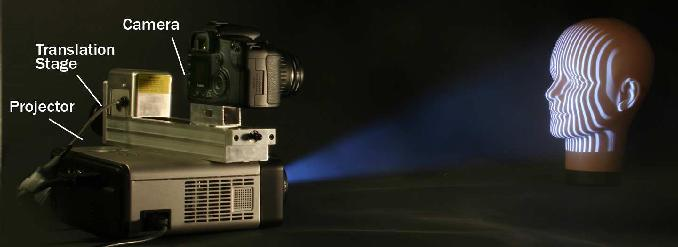
\includegraphics[width=\linewidth]{pictures/structured_light.jpg}
	\caption[Vision-based recognition by structured light.]{Vision-based gesture recognition can be achieved by a structured light approach.
		With structured light the depth information is obtained by projecting a pattern of structured light, 
		and look at the way this pattern deforms when hitting a surface (such as the doll's face in the picture). Picture from~\citet{Ramamoorthi2007}}
	\label{fig:structured_light}
\end{figure} 

As mention previously, these techniques require more processing than those of contact-based devices, but usually allows its user to use the system
without using any form of gloves or armbands~\citep{Rautaray2015}. 
Even though vision-based gesture recognition technologies are more complex, computationally demanding, and prone to 
errors in the form of inaccurate readings, they still have some important advantages over contact-based devices, as will be covered in the next section.

% The Leap Motion Controller is a small USB peripheral device which is designed to be placed on a physical desktop, 
% facing upward. Using two monochromatic IR cameras and three infrared LEDs, the device observes a roughly hemispherical area, to a distance of about 1 meter, 
% and generates almost 200 frames per second of reflected data~\citep{LeapMotion2016}.

\subsection{Technology Comparison}
Both contact-based and vision-based technologies have their advantages and disadvantages (see~\citet{Rautaray2015} for a deeper discussion of these). 
As contact-based devices avoid several of the challenges of vision-based devices, such as illumination and occlusion, they generally have a higher accuracy of recognition.
In addition to this, and as explained earlier, contact-based devices usually also relies less on processing resources as the sensor data can be applied more directly than the
frames captured by a vision-based system. Contact-based systems are also known to give more tactile feedback\footnote{A (simulated) sense of touch to indicate that the user e.g~
has pushed a button} then vision based systems.

Vision-based devices are on the other hand seen as more user friendly, as they usually don't require the user to wear anything, and can thus also be used more easily
in combination with other input methods (such as mouse and keyboard). This is perhaps especially relevant when it comes to using gesture recognition technology in
sterile environments (such as in surgery), as no contact with the device is required. 

The main disadvantage of contact-based devices is the potential health hazards, which may be caused by some of its components~\citep{Schultz2003}. 
Research has suggested that mechanical sensor materials may raise symptoms of allergy and magnetic component may raise the risk of cancer~\citep{Nishikawa2003}. 
Even though vision-based devices have the initial challenge of complex configuration and implementations, 
they are still considered more user friendly and hence more suited for usage in long run. 
Because of these reasons the design review application should thus ideally utilize a vision-based gesture recognition technology. 

Of the three vision-based technologies outlined above, stereoscopic vision is arguably the most promising one~\citep{Ko2012}.
One of the reasons for this is that devices utilizing this technology have proved more reliable in variable light condition than their counterparts, 
as both structured light- and time of flight technologies relies heavily on light to obtain depth information, while stereoscopic vision does so by looking at image offsets.
Stereoscopic vision devices also usually have a better range, i.e they can capture objects farther away from the cameras, and 
a lower material cost (they are cheaper, which also makes them more attractive for the consumer market)~\citep{Ko2012}.
Because of this the stereoscopic vision technology is deemed the most appropriate vision-based technology to use with the design review application.
In the next sections we will review central concepts when utilizing a vision-based gesture recognition system.

% \section{The Primary Vision-based Technologies}
% Today, there are three primary vision-based technologies that can acquire 3D images: Stereoscopic vision, structured light pattern and time of flight (TOF)~\citep{Ko2012}.
% These all make use of one or several cameras and lights to capture and recognize certain movements or poses from the user, 
% and transform it to a certain action on the computer (e.g.~a recognized finger tap might be the equivalent to left mouse button click). 
% 
% \subsection{Stereoscopic Vision}
% Stereoscopic Vision is the most common 3D acquisition method and uses two cameras to obtain a left and right stereo image. 
% These images are slightly offset on the same axis as the human eyes. As the computer compares the two images, 
% it develops a disparity image that relates the displacement of objects in the images.
% 
% \subsection{Structured Light}
% Structured Light measure or scan 3D objects through illumination. Light patterns are created using either a projection of lasers or LED light 
% interference or a series of projected images. 
% By replacing one of the sensors of a stereoscopic vision system with a light source, structured-light-based technology basically exploits the same triangulation as a 
% stereoscopic system does to acquire the 3D coordinates of the object. 
% Single 2D camera systems with an IR- or RGB-based sensor can be used to measure the displacement of any single stripe of visible or IR light, 
% and then the coordinates can be obtained through software analysis.
% 
% \subsection{Time of Flight}
% Time of Flight is a relatively new technique among depth information systems
% and is a type of light detection and ranging (LIDAR) system that transmits a light pulse from an emitter to an object. 
% A receiver determines the distance of the measured object by calculating the travel time of the light pulse from the emitter to the object and back to the receiver 
% in a pixel format.
% 

% 
% \subsection{Comparing the Technologies} 
% Stereoscopic vision is perhaps the most promising one for the consumer market as it has the lowest material cost~\citep{Ko2012}, 
% and has proved more reliable in variable light conditions than its counterparts. 
% One of the latest consumer-oriented devices of this kind is the Leap Motion Controller, 
% which distinguishes itself for having a higher localization precision than other depth vision-based devices~\citep{Weichert2013}, 
% and also for capturing depth data related to palm direction, fingertips positions, palm center position, and other relevant points~\citep{Wei2016}. 
% The Leap Motion Controller will be reviewed more in-depth in chapter~\ref{technical}. 
